\chapter{Tasks}

\subsubsection{I task più comuni sono:}

\begin{itemize}
  \item \fancyglitter{classificazione};
  \item \fancyglitter{Punteggio e classifica};
  \item \fancyglitter{Stima probabilistica};
  \item \fancyglitter{Regressione}.
\end{itemize}

\section{Classificazione}

\dfn{classificazione}{
  La classificazione è il task in cui si ha come obiettivo la costruzione di un modello \^c: $\bbX \to \bbC$ in cui $\bbC = \{C_1, C_2, ..., C_k\}$. Questo modello è un'approssimazione
   del mondo reale. 

   Un esempio è una coppia $(x, c(x)) \in \bbX x \bbC$.  
}

\clm{Il problema dell'induzione}{}{
  L'induzione partendo dai dati di un dataset è generalmente infondata senza ulteriori informazioni.
}

\nt{Il mondo non è semplice, per cui il rasoio di Occame non sempre funziona. Spesso però si utilizzano preconcetti e bias induttivi per avere apprendimento automatico.}

\dfn{classificazione binaria}{
  La classificazione binaria è il caso in cui si hanno solo 2 opzioni (spesso 0 e 1).
}

\nt{Dalla classificazione binaria si può passare alla classificazione multi-classe senza sviluppare nuovi algoritmi.}

  
  \begin{center} 
    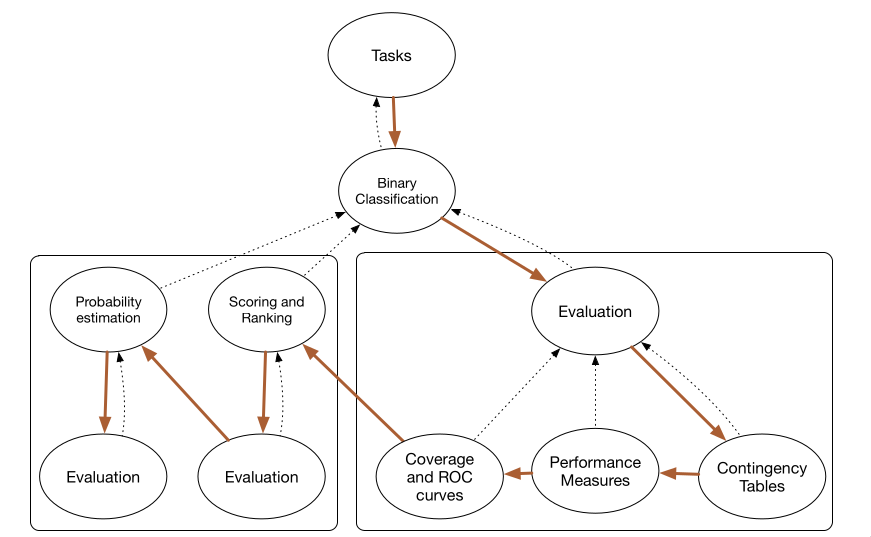
\includegraphics[scale=0.5]{01-Introduzione/Graph.png}
  \end{center}

\dfn{Alberi di decisione}{
  Alberi per visualizzare i dati. Ogni nodo corrisponde a una features.
}

\dfn{Alberi di Features}{
  Alberi per visualizzare i dati. Si ha una suddivisione dei vari esempi divisi per etichette.
}


\begin{center} 
 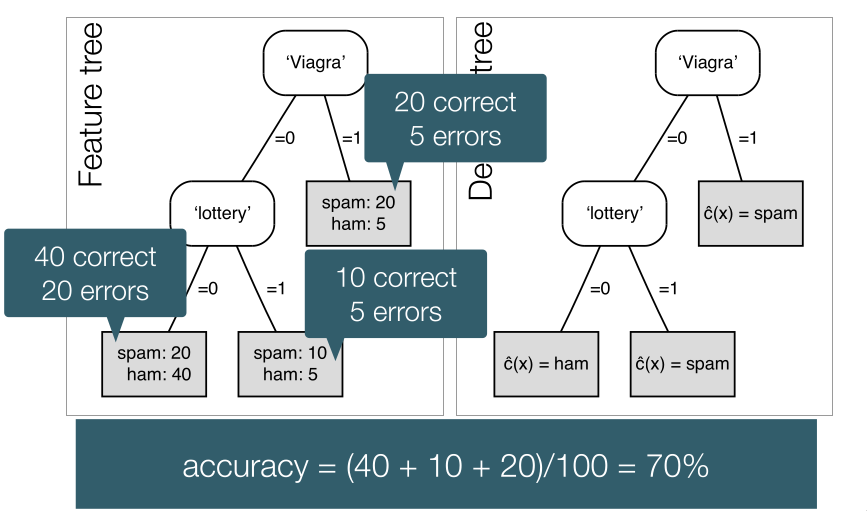
\includegraphics[scale=0.5]{01-Introduzione/AD.png}
\end{center}

\dfn{Tavola di contingenza}{
  Tavola in cui le colonne corrispondono alle predizioni e le righe al mondo reale. Nella loro intersezione si ha il numero di esempi predetti in un certo modo e hanno una certa etichetta (TP, TN, FT, FN).
}


\begin{center} 
 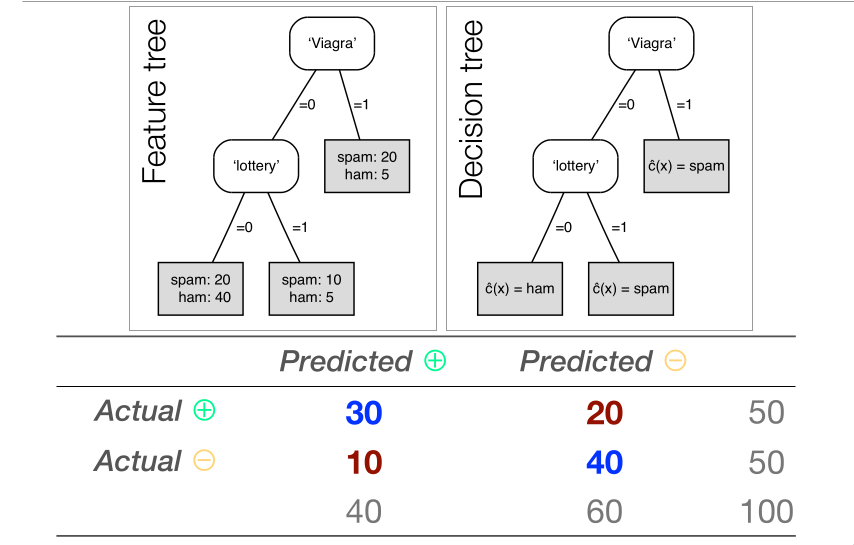
\includegraphics[scale=0.5]{01-Introduzione/TC.png}
\end{center}

\dfn{Grafico di copertura}{
  Grafico per visualizzare le informazioni della tavola di contingenza.
}


\begin{center} 
 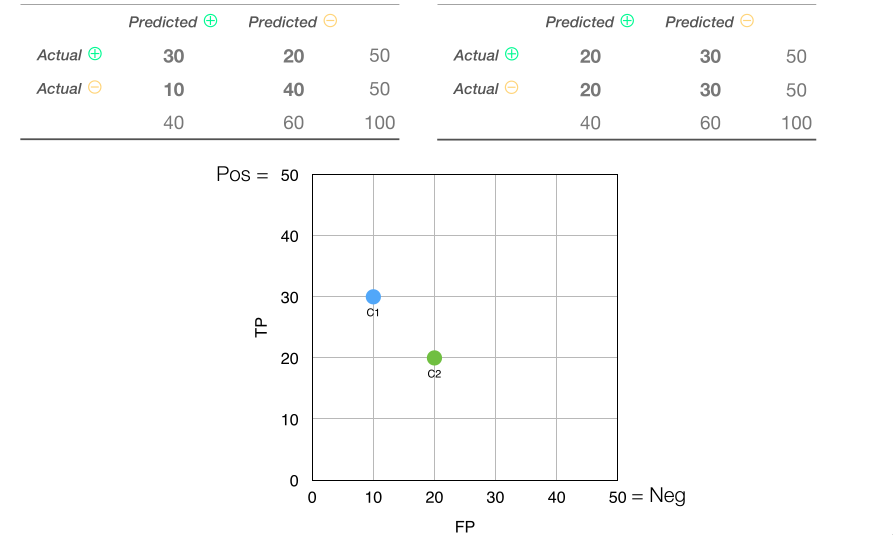
\includegraphics[scale=0.5]{01-Introduzione/GC.png}
\end{center}

\nt{I classificatori che si trovano sulla bisettrice del piano cartesiano sono imprevedibili e quindi poco interessanti. Più un classificatore ha la coordinata x bassa e y alta più è preciso.}

\begin{figure}[h]
  \centering
  \begin{minipage}{0.45\textwidth}
    \centering
    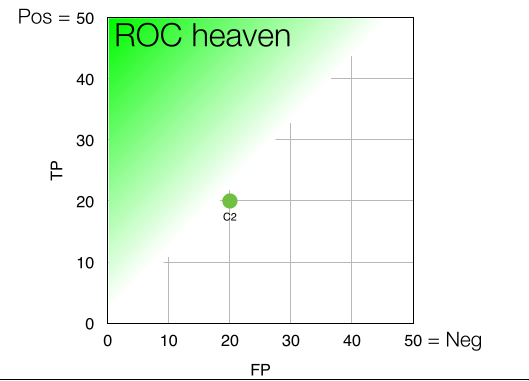
\includegraphics[scale=0.47]{01-Introduzione/ROCHEAVEN.png}
  \end{minipage}\hfill
  \begin{minipage}{0.45\textwidth}
    \centering
    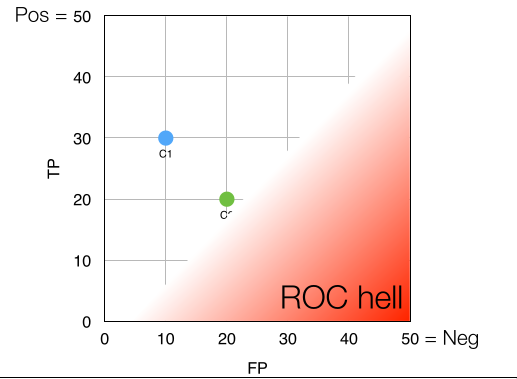
\includegraphics[scale=0.47]{01-Introduzione/ROCHELL.png}
  \end{minipage}
\end{figure}

\nt{Tutti i classificatori che stanno su una retta con pendenza 1 hanno la stessa \fancyglitter{accuratezza}.}

\dfn{Avg recall}{
  \newfancyglitter{avg recall} = (recall + specificity) / 2 = (TP/POS + TN/NEG)/2

  Se due classificatori hanno la stessa avg recall allora sono su linee parallele alla diagonale principale.
}

\begin{center} 
 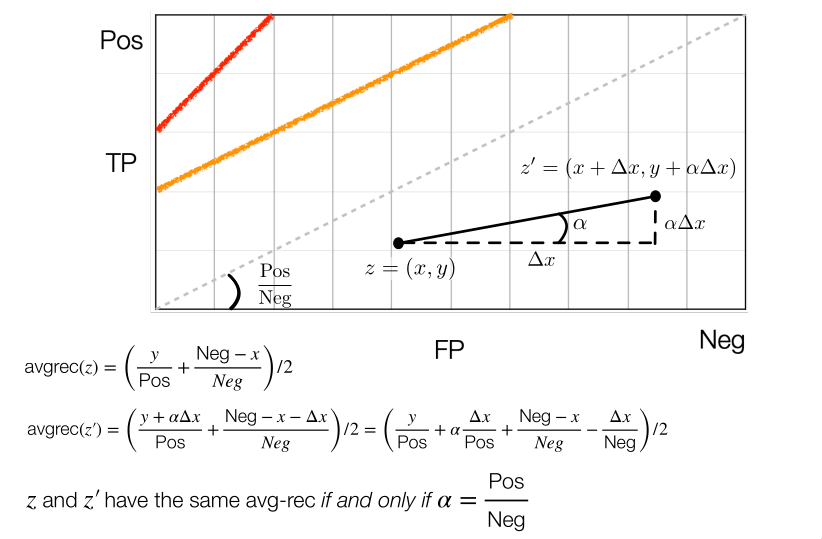
\includegraphics[scale=0.5]{01-Introduzione/avg.png}
\end{center}

\subsection{Roc Plots Properties}

Se si vogliono confrontare le performance di un classificatore su un dataset o su un altro si deve \fancyglitter{normalizzare} gli assi dividendo l'asse x per il numro di esempi negativi e l'asse y per il numero di esempi positivi. Così facendo si otterrà un quadrato con gli assi compresi tra 0 e 1.

\begin{center} 
 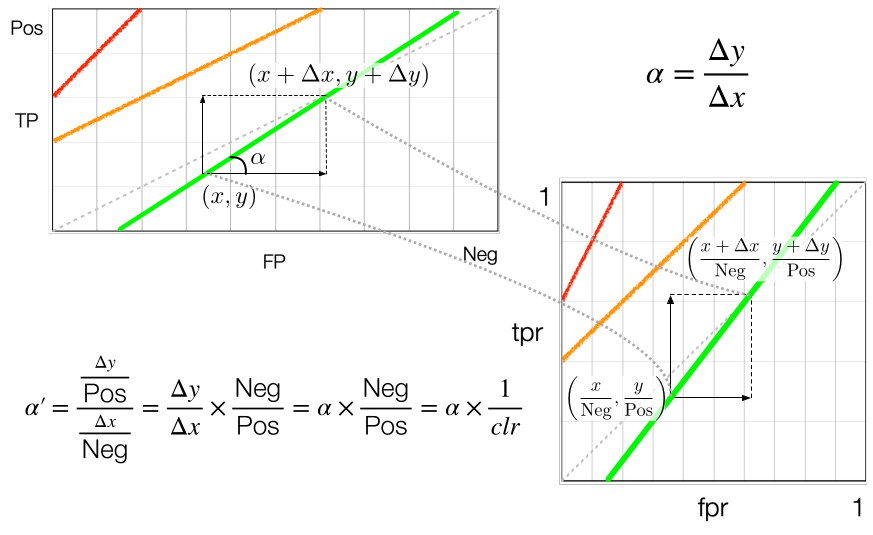
\includegraphics[scale=0.5]{01-Introduzione/Trasl.png}
\end{center}

\nt{Il clr è il class ratio.}

\subsection{Più di un Classificatore per una Singola Feature.}

\begin{center} 
 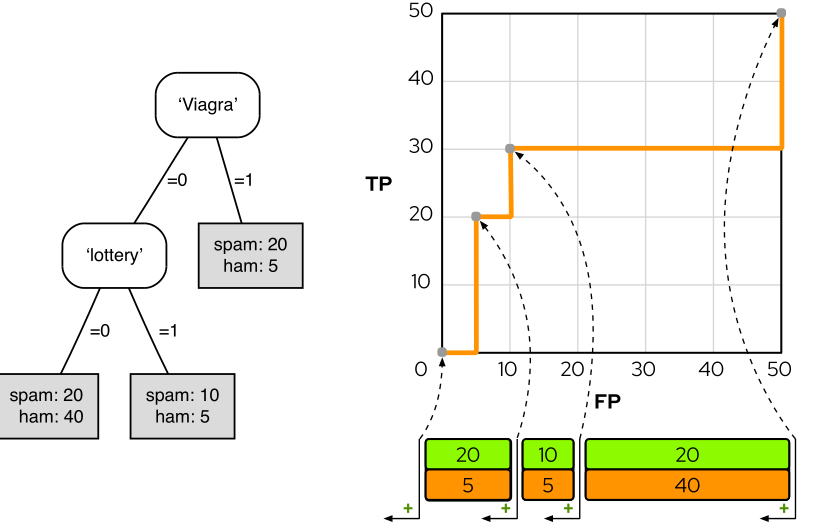
\includegraphics[scale=0.53]{01-Introduzione/MDT.png}
\end{center}

\qs{}{Come si considera il caso in cui il costo per FP (falsi positivi) e FN (falsi negativi) sono differenti?}

\begin{center} 
 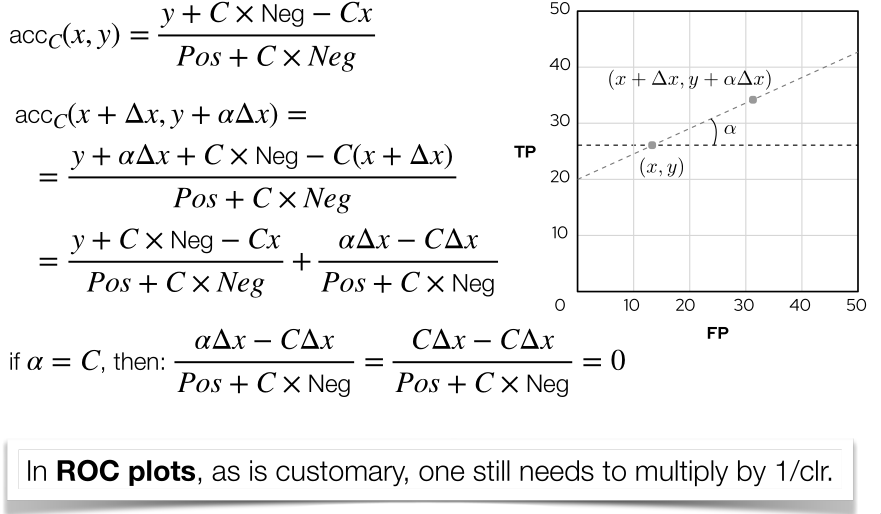
\includegraphics[scale=0.53]{01-Introduzione/FPFN.png}
\end{center}

\section{Scoring e ranking}

\dfn{Scoring classifier}{
  Uno scoring classifier è una mappatura \^s: $\bbX \to \bbR^k$ il cui output è un vettore (\^s (x) = \^s1(x),...,\^si(x)) dove i-esimo componente è lo score assegnato alla classe Ci per l'istanza x.
}

\nt{Se si hanno solo due classi si può considerare solo uno score. Gli score vanno interpretati nel contesto di un classificatore, sono misure della confidenza in una determinata predizione.}

\begin{center} 
 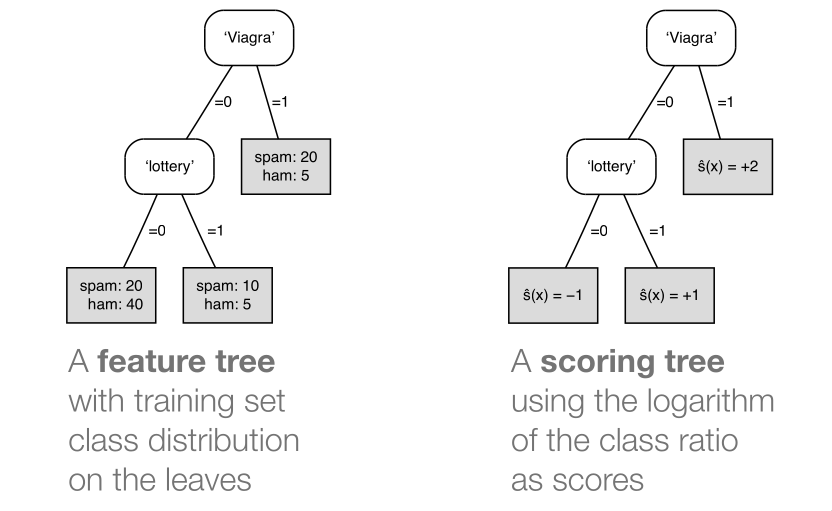
\includegraphics[scale=0.35]{01-Introduzione/ST.png}
\end{center}

\dfn{Margine}{
  Il margine assegnato dallo scoring classifier è positivo se \^s è corretto, negativo altrimenti. Il margine è il prodotto tra la classe dell'esempio e lo score.

  $$z(x) = c(x)\text{\^s}(x) =  \begin{cases}
  z(x) > 0 & \text{se la classificazione è corretta (cioè, } c(x) \text{ corrisponde alla classe prevista)} \\
  z(x) < 0 & \text{se la classificazione è incorretta (cioè, } c(x) \text{ non corrisponde alla classe prevista)} \\
  z(x) = 0 & \text{se lo score è esattamente al confine di decisione}
  \end{cases}$$

}

\subsection{Loss Function}

\dfn{Loss Function}{
  La funzione di loss cerca di pesare l'impatto degli esempi negativi. In 0 la funzione di loss vale 1, tende a infinito con margini molto piccoli (molto negativi).
  \[
  L: \mathbb{R} \to [0, \infty)
  \]
}

\nt{Le loss function sono importanti durante l'apprendimento perché sono usate per guidare la ricerca della soluzione ottimale. }

\subsubsection{Tipi di loss}

\cor{0-1 loss}{
  Si perde un'unità se si sbaglia e non si perde nulla se si indovina.
}

\begin{center} 
 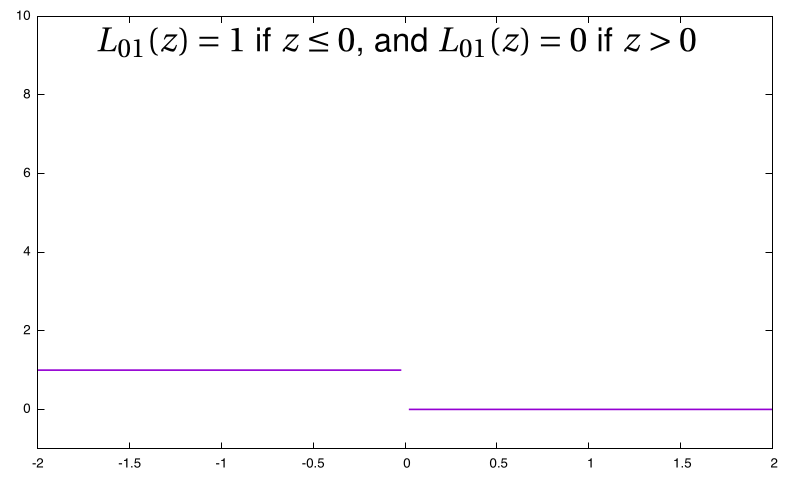
\includegraphics[scale=0.53]{01-Introduzione/01Loss.png}
\end{center}
\pagebreak
\cor{Hinge loss}{
  La Hinge loss è una loss che è lineare per valori minori di 1 e vale 0 per valori maggiori di 1.
}

\begin{center} 
 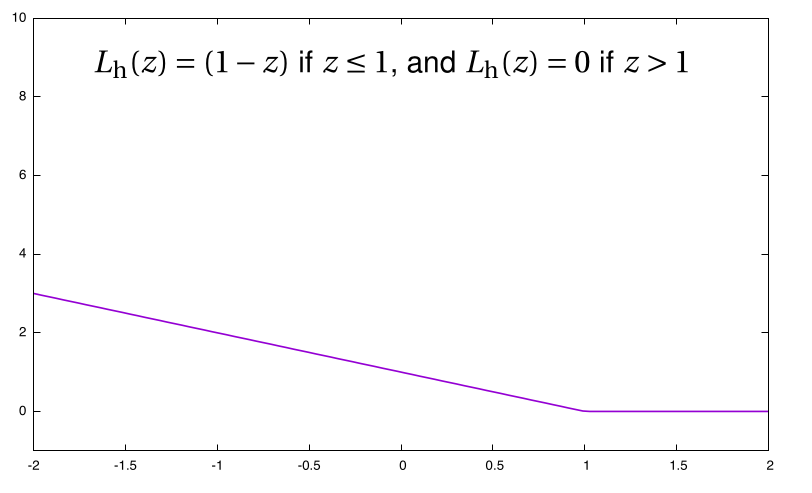
\includegraphics[scale=0.53]{01-Introduzione/Hinge loss.png}
\end{center}

\cor{Logistic loss}{Approssimazione continua della Hinge loss.}

\begin{center} 
 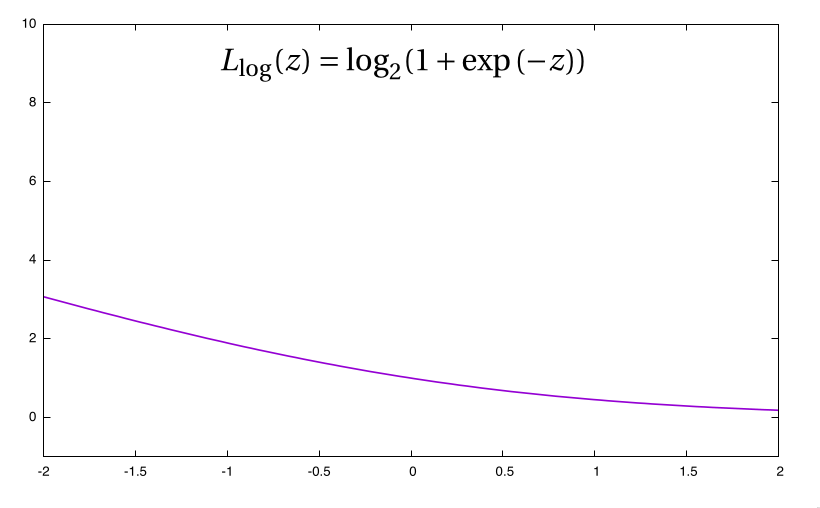
\includegraphics[scale=0.53]{01-Introduzione/Logistic loss.png}
\end{center}

\cor{Loss esponenziale}{Cresce rapidamente quando si stanno facendo errori.}

\begin{center} 
 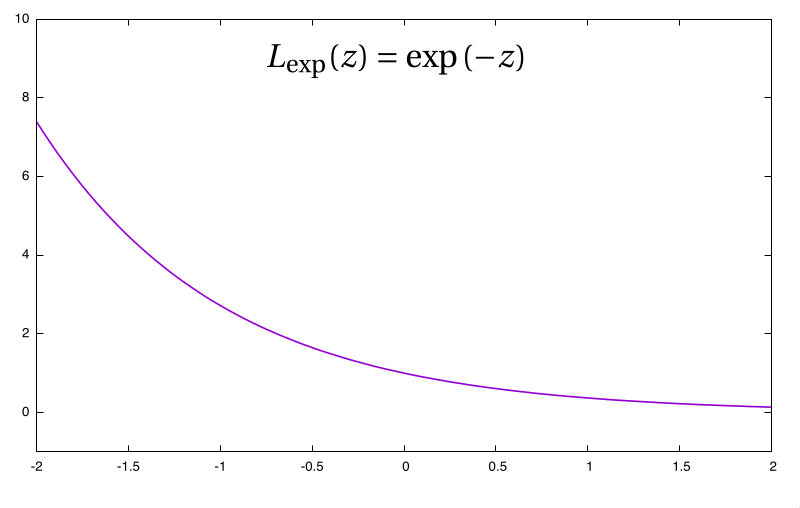
\includegraphics[scale=0.53]{01-Introduzione/Exp Loss.png}
\end{center}

\cor{Loss quadratica}{Se viene ottimizzata troppo si hanno modelli incogniti, funziona meglio con la regressione.}

\begin{center} 
 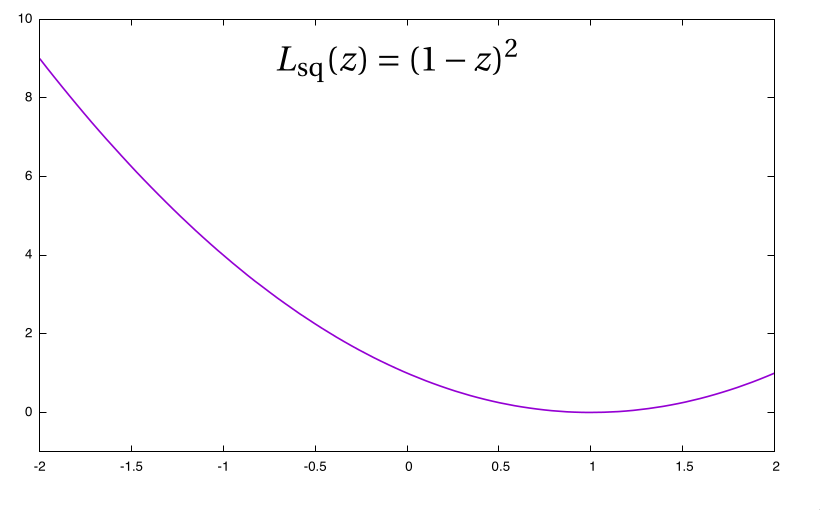
\includegraphics[scale=0.53]{01-Introduzione/Quad loss.png}
\end{center}

\subsection{Ranking}

\dfn{Ranking}{Ordina sulla base di uno score. Dall'esempio che è di classe più positiva a quello di classe meno positiva.}

\cor{Ranking Error Rate}{
\begin{center} 
 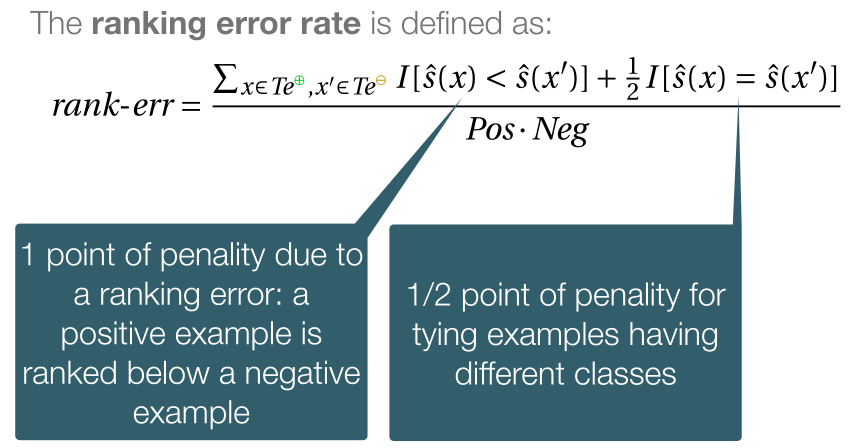
\includegraphics[scale=0.53]{01-Introduzione/Rank.png}
\end{center}
}

\ex{Ranking Error Rate}{
\begin{center} 
 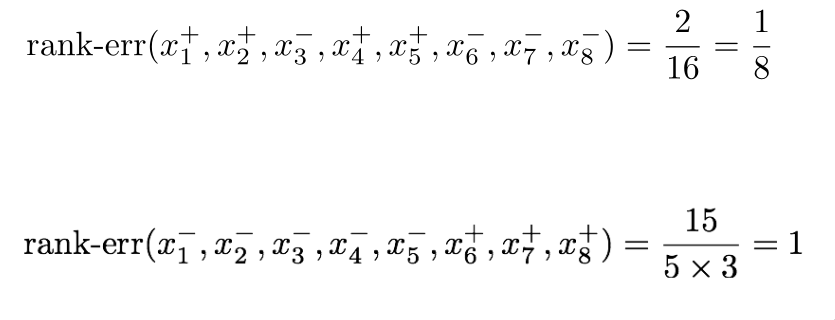
\includegraphics[scale=0.53]{01-Introduzione/Rank1.png}
\end{center}

}
\pagebreak
\ex{Spam}{
  \begin{center} 
 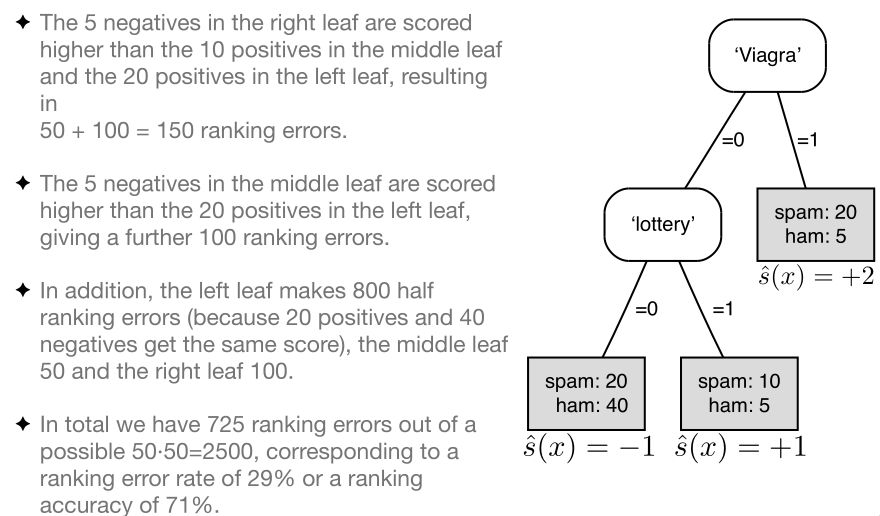
\includegraphics[scale=0.53]{01-Introduzione/Spam6.png}
\end{center}

}

\section{Stima Probabilistica}

\dfn{Stimatore probabilistico di classi}{
  Uno stimatore probabilistico di classi è un classificatore di scoring il cui output è un vettore di probabilità. 

  \[
    \hat{p}: \bbX \to [0, 1]^k
  \]

Scriviamo:

\[
  \hat{p}(x) = (\hat{p}_1(x),\dots,\hat{p}_k(x))
\]

dove l'i-esimo componente è la probabilità assegnata alla classe $C_i$ e $\displaystyle\sum_{i=1}^{k}\hat{p}_i(x) = 1$
}

\nt{Se si hanno solo 2 classi allora \^p(x) denota la probabilità stimata per le classi positive.}

  \begin{center} 
    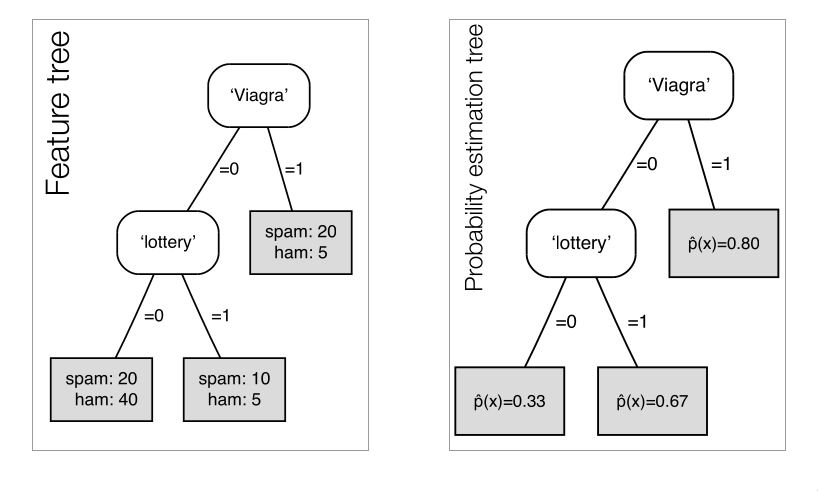
\includegraphics[scale=0.53]{01-Introduzione/prob.png}
\end{center}
\subsection{Squared Error}
\cor{Squared Error}{
    \begin{center} 
 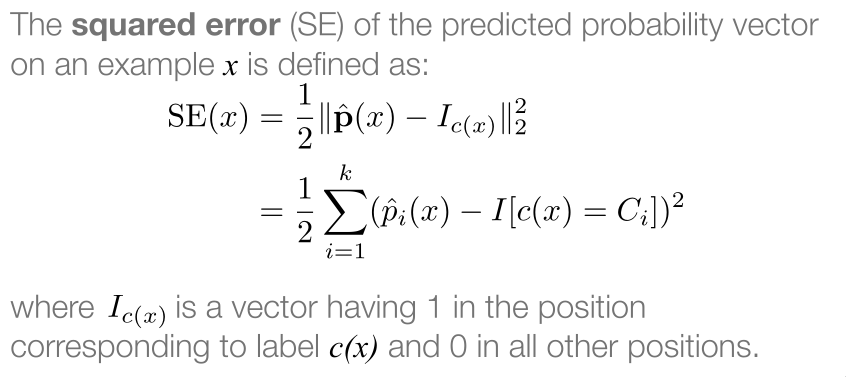
\includegraphics[scale=0.4]{01-Introduzione/SE.png}
\end{center}
}

\cor{Mean Squared Error}{
 Il mean squared error è la media aritmetica degli squared error.
}

\dfn{Probabilità Empiriche}{
  Le probabilità empiriche consentono di ottenere probabilità stimate da classificatori o rankers. Se si ha un insieme S di esempi etichettati e il numero di esempi in S di classe $C_i$ è scritto $n_i$ il vettore di probabilità empiriche associato ad S sarà:

  \[
    \hat{p}(S) = (n_1/|S|,\dots, n_k/|S|)
  \]
}
\pagebreak
\cor{Correzione di Laplace}{
  Se si ha un insieme S e dentro si hanno $n_i$ elementi di classe $C_i$ per ogni classe si fa finta di avere un esempio aggiuntivo.

  \[
    \hat{p}_i(S) = \frac{n_i + 1}{|S| + k}
  \]

Si può applicare anche:

  \[
    \hat{p}_i(S) = \frac{n_i + m*\pi_i}{|S| + m}
  \]
La Correzione di Laplace è un caso speciale in cui $m = k$ e la distribuzione è uniforme ($\pi_i = \frac{1}{k}$)
}

\section{Oltre la Classificazione Binaria}

\begin{figure}[h]
  \centering
  \begin{minipage}{0.45\textwidth}
    \centering
    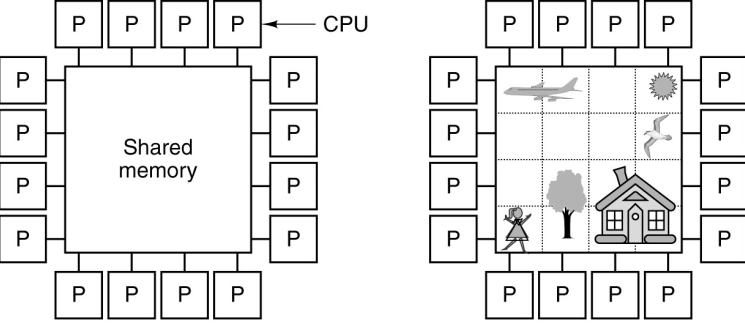
\includegraphics[scale=0.3]{01-Introduzione/Multi.png}
  \end{minipage}\hfill
  \begin{minipage}{0.45\textwidth}
    \centering
    
\includegraphics[scale=0.3]{01-Introduzione/NB.png}
  \end{minipage}
\end{figure}

\subsubsection{Schemi per estendere la classificazione binaria al caso multi-classe:}

\begin{itemize}
  \item one-vs-rest:
    \begin{itemize}
      \item apprendimento non ordinato;
      \item apprendimento in ordine fisso.
    \end{itemize}
  \item one-vs-one:
    \begin{itemize}
      \item simmetrici;
      \item asimmetrici.
    \end{itemize}
\end{itemize}

\subsubsection{One-vs-Rest (non ordinato)}

\begin{center} 
 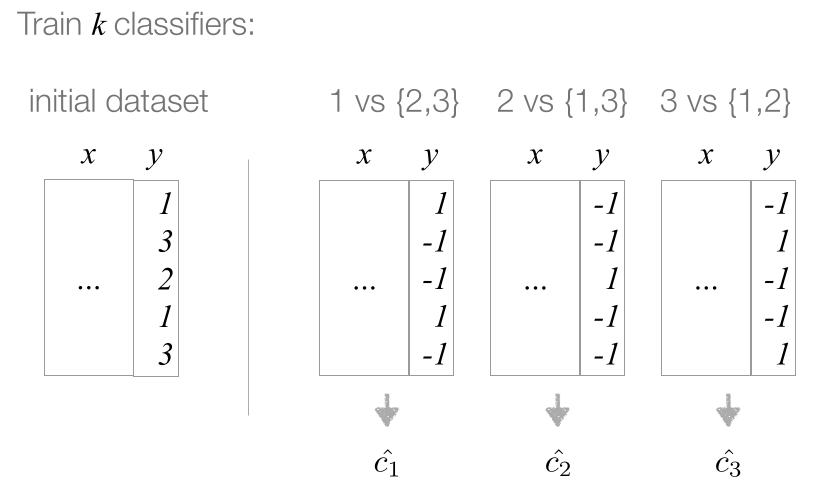
\includegraphics[scale=0.5]{01-Introduzione/ovro.png}
\end{center}

\nt{Si può costruire una matrice con il codice di output: in ogni riga si mette una classe, in ogni colonna si mette un classificatore che si vuole costruire e in ogni cella il valore che si vuole in output.}

\begin{center} 
 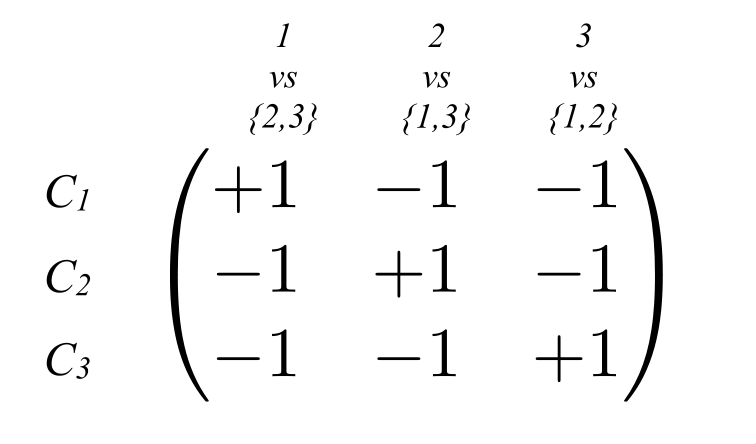
\includegraphics[scale=0.35]{01-Introduzione/ovro1.png}
\end{center}

\subsubsection{One-vs-Rest (ordinato)}

\begin{center} 
 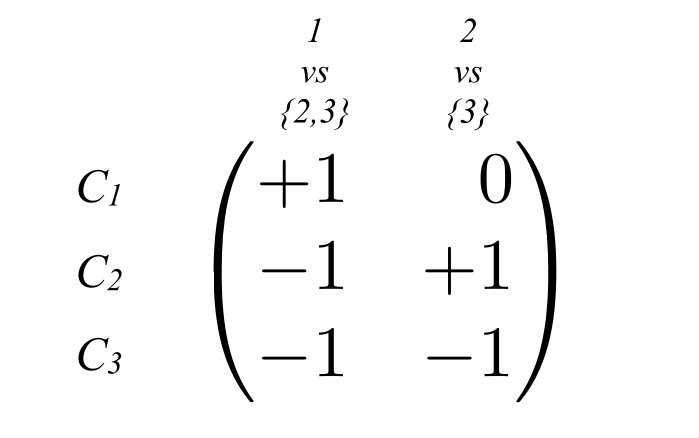
\includegraphics[scale=0.35]{01-Introduzione/ovro2.png}
\end{center}

\subsubsection{One-vs-one (simmetrico)}

\begin{center} 
 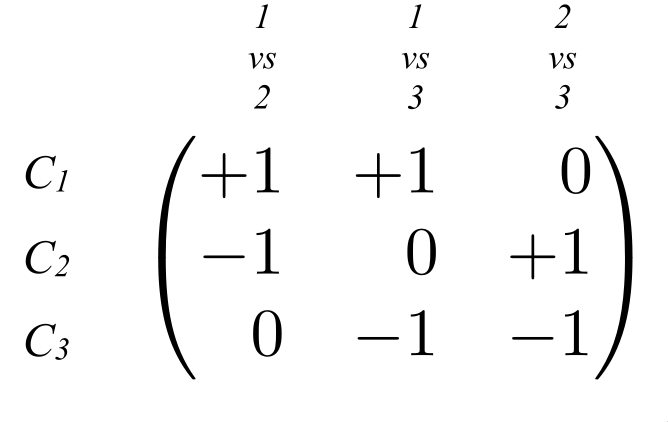
\includegraphics[scale=0.35]{01-Introduzione/ovos.png}
\end{center}

\subsubsection{One-vs-one (asimmetrico)}

\begin{center} 
 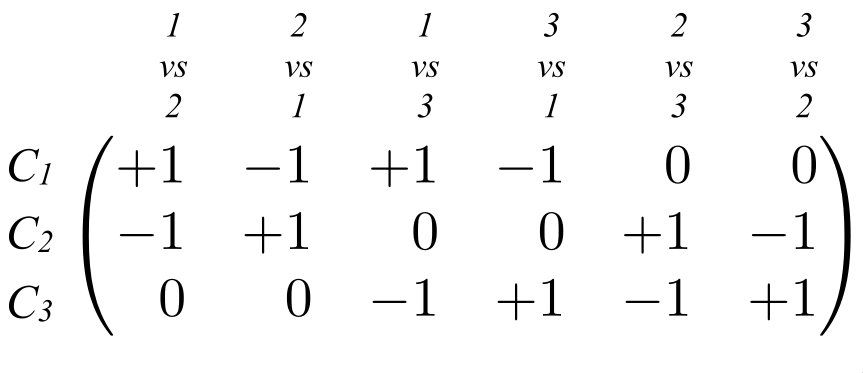
\includegraphics[scale=0.35]{01-Introduzione/ovoa.png}
\end{center}

\nt{Per classificare un nuovo esempio (vettore) si cerca la riga più simile.}

\clm{Difficoltà nell'applicare one-vs-rest e one-vs-one}{}{

  \begin{itemize}
    \item   Nel caso one-vs-rest il singolo classificatore vede un dataset molto sbilanciato sebbene il dataset di partenza fosse bilanciato. 
    \item Nel caso one-vs-one il problema è mitigato assegnando 0 agli esempi che non appartengono alle due etichette scelte. Però è problematico quando si ha scarsità nei dati. 
  \end{itemize}
}

\qs{}{Come si rompono i pareggi?}

\begin{enumerate}
  \item Si aggiungono classificatori;
  \item Se si ha un algoritmo di apprendimento in grado di assegnare uno score si può scegliere il valore su cui si è più confidenti.
\end{enumerate}

\subsection{Regressione}

\dfn{Stimatore di funzione}{
  Uno stimatore di funzione, chiamato \newfancyglitter{regressore}, è una mappatura:

  \[
    \hat{f} : \bbX \to \bbR
  \]
  Il problema dell'apprendimento con la regressione è imparare uno stimatore di funzione dagli esempi $(x_i, f(x_i))$
}

\nt{In questo caso, a differenza dei precedenti, si passa a etichette di tipo reale (infinito non numerabile).}

\subsubsection{Funzione continua}

\begin{center} 
 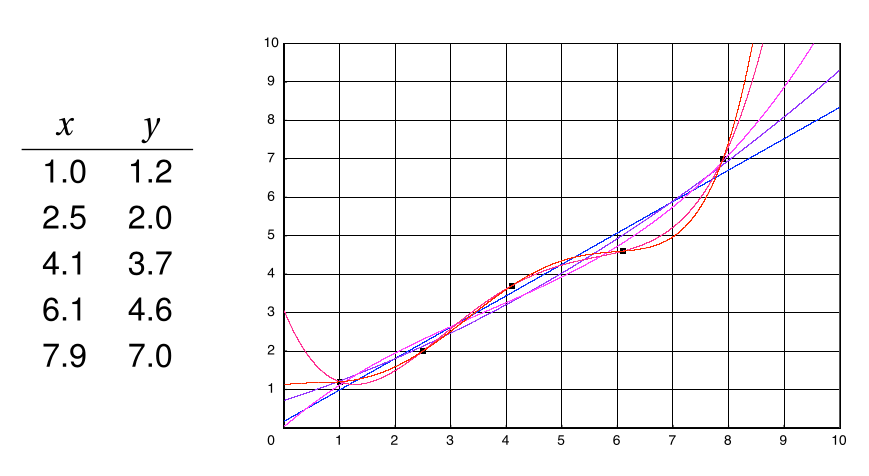
\includegraphics[scale=0.45]{01-Introduzione/PD.png}
\end{center}

\subsubsection{Funzione costante a tratti}

\begin{center} 
 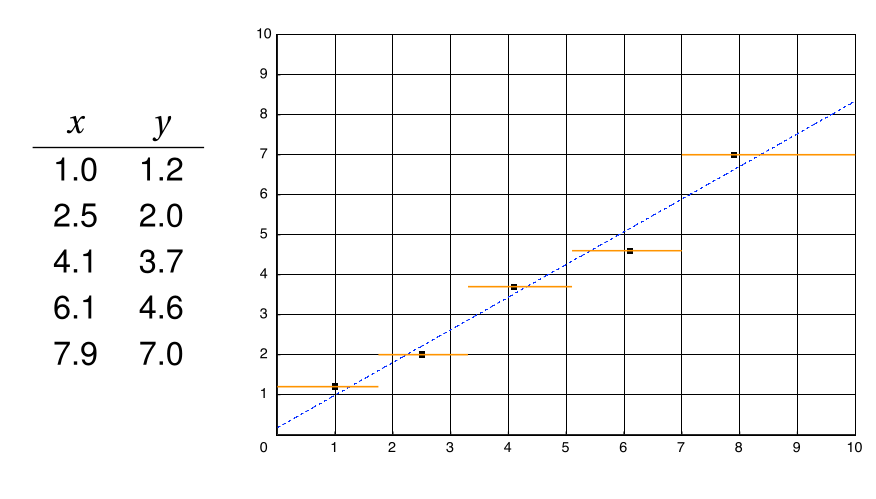
\includegraphics[scale=0.45]{01-Introduzione/PD1.png}
\end{center}

\nt{
  Se si vuole "fittare" n + 1 punti si può utilizzare un polinomio di grado n (quindi con n + 1 parametri). 

  Per evitare l'overfitting il numero dei parametri stimati dai dati deve essere molto minore del numero dei punti. 
}

\dfn{Bias-Variance Dilemma}{
  Un  modello a bassa complessità si ha bassa variabilità a causa della variazione casuale nei dati. Però viene introdotto un bias sistematico che nemmeno un modello più grande può risolvere. 

  Un modello ad alta complessità elimina questo bias, ma è soggetto a errori dovuti alla varianza.

\[
  E[(f - \hat{f})^2] = (f - E[\hat{f}])^2 + E[(\hat{f} - E[\hat{f}])^2] = Bias^2(\hat{f}) + Var(\hat{f})
\]

\begin{itemize}
  \item $(f - E[\hat{f}])^2$, zero se il regressore è mediamente corretto, altrimenti ha un bias sistematico;
  \item $E[(\hat{f} - E[\hat{f}])^2]$, errore dovuto alla fluttuazione attorno alla media (errore dovuto alla varianza).
\end{itemize}

}

\begin{center} 
 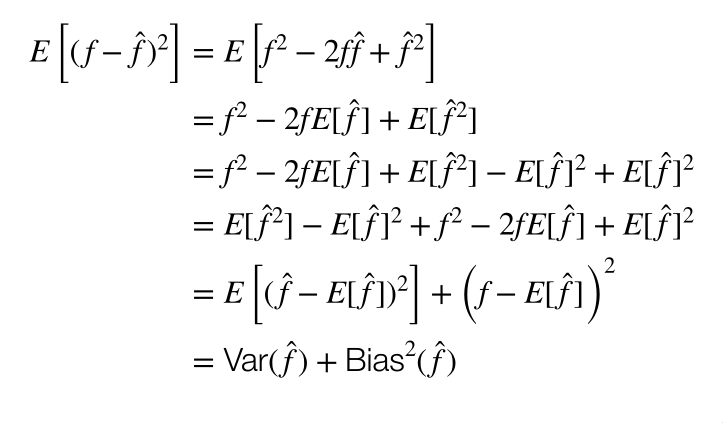
\includegraphics[scale=0.45]{02-Tasks/BV.png}
\end{center}
\cor{Bias}{
  Errore sistematico dovuto al fatt che il modello on è in grado di "fittare" perfettamente i dati (e.g. si sta cercando di "fittare" una parabola usando una retta).
}

\cor{Variance}{
  Errore per cui i modelli sono instabili (si ha del rumore). Anche con una minima variazione il modello può cambiare completamente.
}

\subsection{Apprendimento non Supervisionato}

\dfn{Apprendimento non Supervisionato}{
  Nell'\newfancyglitter{apprendimento non supervisionato} non ci sono etichette associate ai dati. Il task consiste nel trovare \newfancyglitter{regolarità} nei dati usando solo i dati stessi.
}

\nt{Un task non supervisionato è il Clustering che può essere sia predittivo che descrittivo.}

\dfn{Clustering}{
  Il task del Clustering è guadagnare maggiore comprensione dei dati dividendo i dati stessi in gruppi tra loro omogenei.
}

\cor{Clustering predittivo}{
  Nel Clustering predittivo si può modellare il problema con la mappatura:
  \[
    \hat{q}: \bbX \to \bbC
  \]

dove $\bbC = \{\bbC_1,\dots, \bbC_k\}$ è un nuovo insieme di etichette.

}

\begin{center} 
 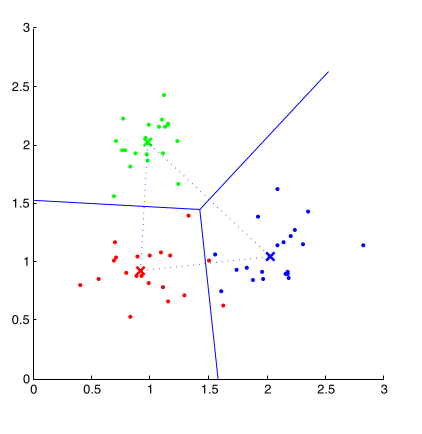
\includegraphics[scale=0.47]{02-Tasks/ClustPred.png}
\end{center}
\cor{Clustering descrittivo}{
  Nel Clustering descrittivo si può modellare il problema con la mappatura:
  \[
    \hat{q}: D \to \bbC
  \]
  dove $D$ è il dataset usato.
}


\begin{center} 
 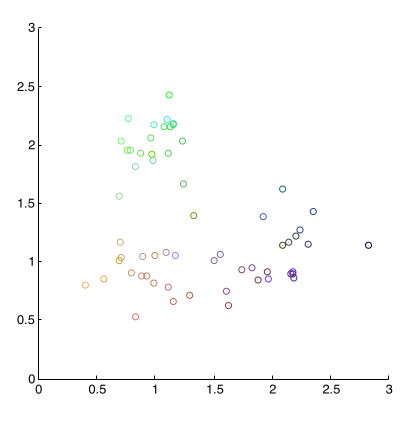
\includegraphics[scale=0.47]{02-Tasks/ClustDesc.png}
\end{center}

\subsection{Subgroup-discovery}

\dfn{Subgroup-discovery}{
  Dato il dataset $\{(x, l(x))\}$ si vuole trovare una funzione:

  \[
    \hat{g} : D \to \{true, false\}
  \]
  tale che $G = \{x \in D | \hat{g}(x) = true\}$ ha una distribuzione di classe molto diversa dalla popolazione iniziale.
}

\nt{$G$ è un \fancyglitter{estensione} del sottogruppo.}

\clm{Subgroup-discovery}{}{
  \begin{itemize}
    \item In generale i Subgroup-discovery sono guidati da una valutazione delle misure;
    \item Tendono a favorire sottogruppi più grandi;
    \item Sono solitamente simmetrici (hanno lo stesso valore sia per il sottogruppo che per il suo completamento);
    \item Il risultato tenderà a dividere lo spazio in due parti uguali.
  \end{itemize}
}

\subsection{Regole di Associazione}

\dfn{Regole di Associazione}{
  Si ha un dataset non etichettato $D$ e si vuole trovare un insieme di regole $\{b \to h\}$ tale che l'oggetto $b \cup h$ sia frequente e che $h$ sia vera quando $b$ è vera, 
}

\nt{$b$ e $h$ sono insieme di coppie attributo/valore.}

\ex{Supermercato}{
  
\begin{center} 
 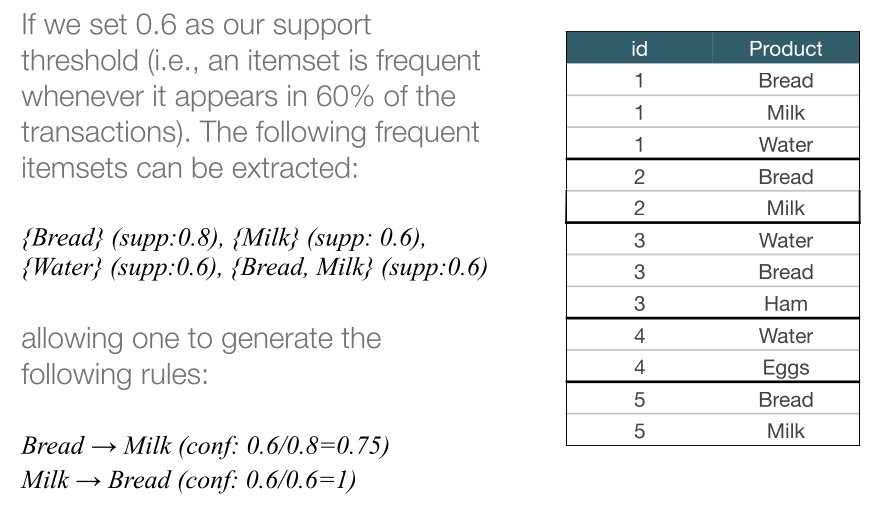
\includegraphics[scale=0.43]{02-Tasks/Supermercato.png}
\end{center}

}












